\documentclass[review]{elsarticle}

\usepackage{lineno,hyperref}
\modulolinenumbers[5]

\journal{Journal of \LaTeX\ Templates}

%%%%%%%%%%%%%%%%%%%%%%%
%% Elsevier bibliography styles
%%%%%%%%%%%%%%%%%%%%%%%
%% To change the style, put a % in front of the second line of the current style and
%% remove the % from the second line of the style you would like to use.
%%%%%%%%%%%%%%%%%%%%%%%

%% Numbered
%\bibliographystyle{model1-num-names}

%% Numbered without titles
%\bibliographystyle{model1a-num-names}

%% Harvard
%\bibliographystyle{model2-names.bst}\biboptions{authoryear}

%% Vancouver numbered
%\usepackage{numcompress}\bibliographystyle{model3-num-names}

%% Vancouver name/year
%\usepackage{numcompress}\bibliographystyle{model4-names}\biboptions{authoryear}

%% APA style
%\bibliographystyle{model5-names}\biboptions{authoryear}

%% AMA style
%\usepackage{numcompress}\bibliographystyle{model6-num-names}

%% `Elsevier LaTeX' style
\bibliographystyle{elsarticle-num}
%%%%%%%%%%%%%%%%%%%%%%%

\usepackage{amsmath}
\usepackage{amsfonts}
\usepackage{booktabs}
\usepackage{subcaption}
\usepackage[export]{adjustbox}
\usepackage{float}

\begin{document}

\begin{frontmatter}

\title{Controlling outer facial features in StyleGAN's latent space operations}

\author[1]{Agustín Roca}
\ead{aroca@itba.edu.ar}

\author[1]{Nicolás Ignacio Britos}
\ead{nbritos@itba.edu.ar}

\affiliation[1]{organization={Instituto Tecnológico de Buenos Aires},
city={Ciudad Autónoma de Buenos Aires},
country={Argentina}}


\begin{abstract}

Previous research has suggested that human recognition of faces rely more in the outer facial features (the contour of the face, ears, chin, and hairline) than the inner facial features (eyes, nose and mouth) for unfamiliar faces. However, there has been little consideration of this when designing the StyleGAN projectors. In this paper, we explore the latent space of StyleGAN to preserve the outer facial features when projecting an image to the latent space or moving through latent directions. Our method involves a post-processing step that modifies the generated images to enhance the preservation of the outer facial features. Our results show that our method is effective in preserving the outer facial features with the tested images.

\end{abstract}

\begin{keyword}
StyleGAN, Generative adversarial network, Latent space, Outer facial features, Image editing, Human perception, Latent directions, Projection
\end{keyword}

\end{frontmatter}

\linenumbers 

\section{Introduction}

Recognizing faces is a fundamental ability for humans, but it's a complex task that depends on various factors. According to several studies, features such as the outer contour of the face, ears, chin, and hairline are the most important when trying to remember unfamiliar faces ~\cite{Want_2003} ~\cite{Young_1985} ~\cite{Bruce_1999} ~\cite{Ellis_1979}  ~\cite{Hancock_2000}. These set of features, is what we refer to as the outer facial features.

Preserving the outer facial features has important implications for various face generation and editing applications, such as face swapping, face aging, and virtual makeup. 

In these applications, the goal is to modify the appearance of a face while keeping its identity intact, or to generate a new face that looks similar to a given face. The outer facial features plays a crucial role in these tasks, as it provides a stable reference for the overall shape and proportions of the face. If the outer facial features is lost or distorted during the editing process, the resulting face may look unrealistic or unrecognizable, which can limit the usability and appeal of the application. By preserving the outer facial features when generating or manipulating faces, we can ensure that the edited faces retain their identity and resemblance to the original faces, which can enhance the user experience and the realism of the results.

The Innocence Project Argentina is an non-profitable organization that is fighting against wrongful convictions in Argentina. One of their lines of work is measuring how effective are eye witnesses when identifying people in police lineups. To do this, they need one of these applications to create different similar faces. Specifically, they want to create different faces while preserving the outer facial features. However, there was no application that actively tries to preserve the outer facial features. It can be done manually with picture editing applications, but would need experts to create realistic results.

For a first approach, they are using StyleGAN~\cite{Karras_2018}~\cite{Karras_2019}, a state-of-the-art generative model for creating realistic face images. StyleGAN's projector allows to input an arbitrary face image, and give a visually similar face in the latent space. Also, when moving the latent code through some specific directions, the image can suffer semantic changes, such us aging, change of orientation and changes in the smile and eyes.

However, despite their importance, the relationship between the outer facial features and the latent space of StyleGAN has received little attention so far. In this paper, we aim to address this by exploring the latent space of StyleGAN to preserve the outer facial features when manipulating the generated images. Specifically, we propose a post-processing step that modifies the generated images to enhance the preservation of the outer facial features.

To do this, we will take advantage of existing neural networks that segments images in three classes: face, hair and background, and use its output to measure the difference of outer facial features between two images. Using this measurement as a loss function, an algorithm can move through the latent space minimizing the outer facial features difference.

We analyze how effective is the proposed correction of the outer facial features for the projection operation and when moving through latent directions. The results show that the method can reduce the outer facial features difference by a considerable amount.

The contributions of this work are: (1) a method to quantify the difference of outer facial features between two faces images, and (2) a proposal to use a post-processing step that modifies the generated images by StyleGAN to enhance the preservation of the outer facial features.

The paper is organised as follows. Section \ref{subsection:outer_features_difference_measurement} describes how we classify the pixels of the image into hair, face and background. Section \ref{subsection:outer_features_difference_formula} defines the function that the algorithm use to measure the outer facial features difference between two images. Section \ref{subsection:outer_features_correction_algorithm} describes the post-processing step that preserves the outer facial features of the original image. The results and their discussion are presented in Section \ref{section:results}. Section \ref{section:conclusions} concludes the paper.

\section{Materials and Methods}\label{section:materials_and_methods}
\subsection{Outer facial features difference measurement}\label{subsection:outer_features_difference_measurement}

The concept of outer facial features has already been introduced as the combination of the contour of the face, ears, chin, and hairline. For example, Figure \ref{fig:outer_facial_features} shows two faces with the same outer facial features.

\begin{figure}[H]
  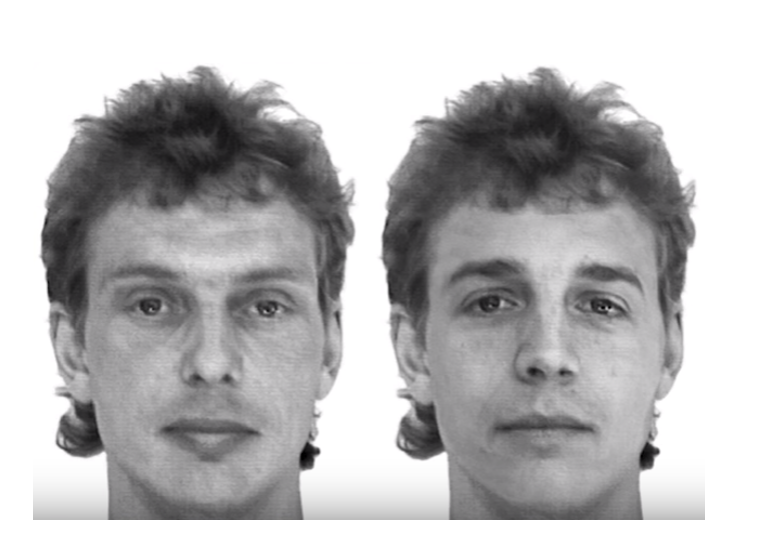
\includegraphics[width=0.5\textwidth, center]{Images/face_frame.png}
  \caption{Two different faces with the same outer facial features.}
  \label{fig:outer_facial_features}
\end{figure}

Having this in mind, we measure the variation of the outer facial features between two images based on the position of the face and hair in the image.

\subsubsection{Image segmentation}
The first thing we need to do is to identify the face and hair inside an arbitrary image. This consists of a simple segmentation problem, separate the pixels of an image in three groups: face, hair and background. For this, an open-source pretrained neural network is used~\citep{Gupta_2018}. 

\subsection{Outer facial features difference formula}
\label{subsection:outer_features_difference_formula}

Once each pixel of each of the two images is classified, we compare the classifications between the pixels in the same position of the two images. Let $f$ be a function that compares the classifications of two pixels,

\begin{equation}
f(c_1, c_2) = 
   \left\{
\begin{array}{ll}
      0 & c_1 = c_2 \\
      0.2 & c_1 = "Face" \land c_2 = "Hair" \\
      0.2 & c_1 = "Hair" \land c_2 = "Face" \\
      1 & otherwise \\
\end{array} 
\right. 
\end{equation}

The number 0.2 is arbitrary, but it means that the face-hair variation is 5 times less important than variations involving the background of the image.

Let $F$ be the function that measures the variation of outer facial features between two images ($I_1$ and $I_2$) of same size, with height $h$ and width $w$. The classifications of the pixels of $I_1$ are $p_{i,j}$, and the classifications of the pixels of $I_2$ are $q_{i,j}$.

\begin{equation}
F(I_1, I_2) = \frac{\sum_{i=1}^{h} \sum_{j=1}^{w} f(p_{i,j}, q_{i,j})}{h*w}
\end{equation}

This function yields a percentage of the images that is classified differently, giving more importance to background variations. If the outer facial features does not vary between two images $I_1$ and $I_2$, then $F(I_1, I_2)=0$. If there is a change in at least one pixel, then $0 < F(I_1, I_2) \leq 1$.

\subsection{Outer facial features correction algorithm}\label{subsection:outer_features_correction_algorithm}

To try to obtain results with the least variation of outer facial features as possible, we propose an algorithm to move around the surroundings of the latent space of the original face to minimize the function defined in \ref{subsection:outer_features_difference_formula}. 

The whole algorithm is very similar to the projection algorithm designed for StyleGAN. The correction takes the target image and a latent code (usually output of projection or result of moving through latent direction) as its input. First, it calculates the standard deviation of 10000 random latent codes that create realistic images, which allows us to apply noise to the original latent code in a way that we can be certain it will yield a realistic image. The $f(target image, G(initial latent code))$ is also calculated and stored in this first step. The noise strength in each iteration is the result of applying the following formula:

\begin{equation}
s(i) = l_{\sigma} * n_0 * (\frac{1-\frac{i}{10000}}{r}) ^{2}
\end{equation}
Being $i$ the current iteration number, $l_{\sigma}$ the standard deviation of the latent codes previously mentioned, $n_0$ a constant representing the initial noise factor, and $r$ a constant representing the noise ramp length. In these experiments, the values are $n_0 = 0.005$ and $r = 0.75$, which follow what StyleGAN2 uses.

Throughout every of the $N$ iterations, the algorithm introduces a Gaussian noise multiplied by $s(i)$ to the latent code. If this new latent code generates an image with less outer facial features variation than the previous latent code, then this new one is stored and used as the current latent code. If that is not the case, the original is preserved. 

Having set fixed values of $n_0 = 0.005$ and $r = 0.75$ taken from StyleGAN, the optimal value of $N$ is studied having in mind the reduction of the outer facial features variation of the target image and the projected one as much as possible.

\section{Results}\label{section:results}

\subsection{Image segmentation}

This network proved to give satisfying results for different faces and images with different conditions. This is essential for the measurement because there is no need to modify any parameters for different images. In Figure \ref{fig:segmentation}, we can see some examples of segmentation made by this network. In yellow the pixels classified as hair; in blue the pixels classified as face; and in purple the pixels classified as background.

\begin{figure}[H]
  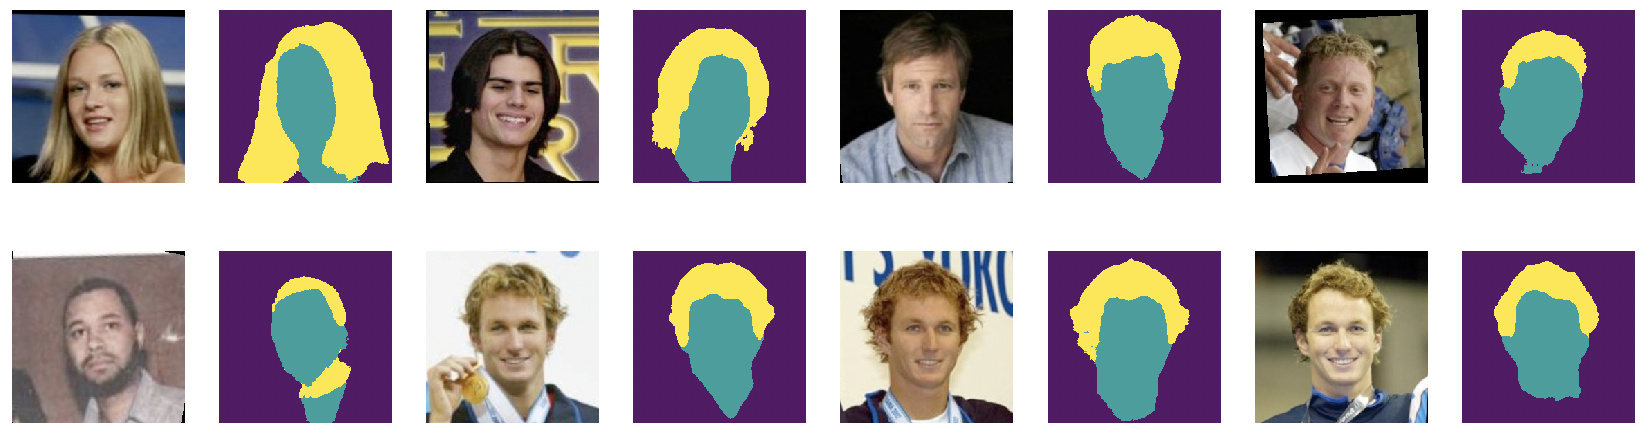
\includegraphics[width=\linewidth, center]{Images/segmentation.png}
  \caption{Segmentation made by the neural network.}
  \label{fig:segmentation}
\end{figure}

\subsection{Fa}

In Figure \ref{fig:correction_demo}, we can see an example of a target face being projected into the latent space as it outputs the neural network and another one after applying the correction algorithm.

\begin{figure}[H]
  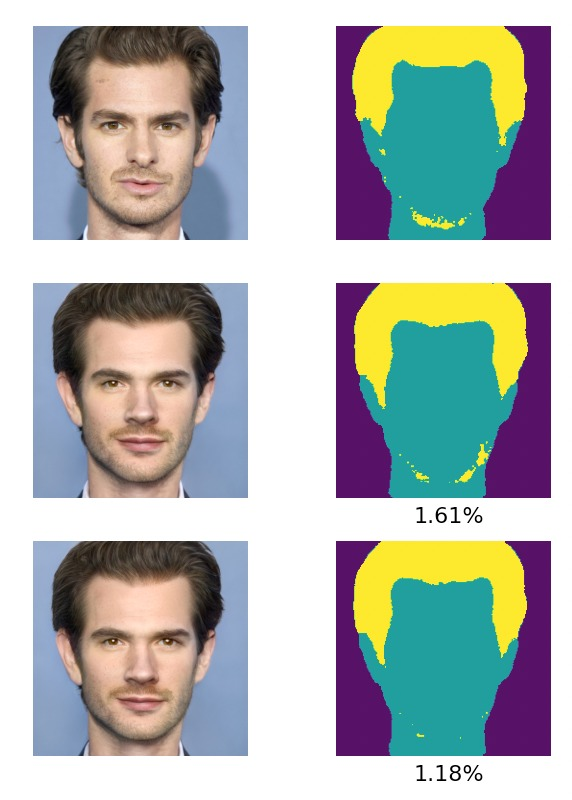
\includegraphics[width=0.5\linewidth, center]{Images/750.jpeg}
  \caption{A target face image (top left), its output from the neural network (top right) and its output after running it through the correction algorithm, with its outer facial features difference.}
  \label{fig:correction_demo}
\end{figure}

\subsection{Projection to latent space}

Table \ref{table:projection} shows the outer facial features difference that the image to latent space projection achieved with each image. The maximum difference is at 3.192\% while the minimum at 0.747\%. The mean difference between these images is of 1.812\%. This results suggest that images are a decent starting point when trying to generate similar faces with minimum outer facial features difference. 

\begin{table}[H]
\begin{tabular}{|l|l|l|l|l|l|l|}
\hline
\textbf{Image} & Andrew & Daniel & Emma & Jennifer & Kristen & Matt \\ \hline
\textbf{Difference} & 1.429\% & 1.894\% & 2.531\% & 1.790\% & 2.267\% & 1.452\% \\ \hline
\end{tabular}

\begin{tabular}{|l|l|l|l|l|l|}
\hline
\textbf{Image} & Paul & Rob & Rosa & Sheldon & Zendaya \\ \hline
\textbf{Difference} & 1.198\% & 2.381\% & 3.192\% & 1.041\% & 0.747\% \\ \hline
\end{tabular}

  \caption{Outer facial features difference results for projecting to latent space}
  \label{table:projection}
\end{table}

\begin{figure}[H]
  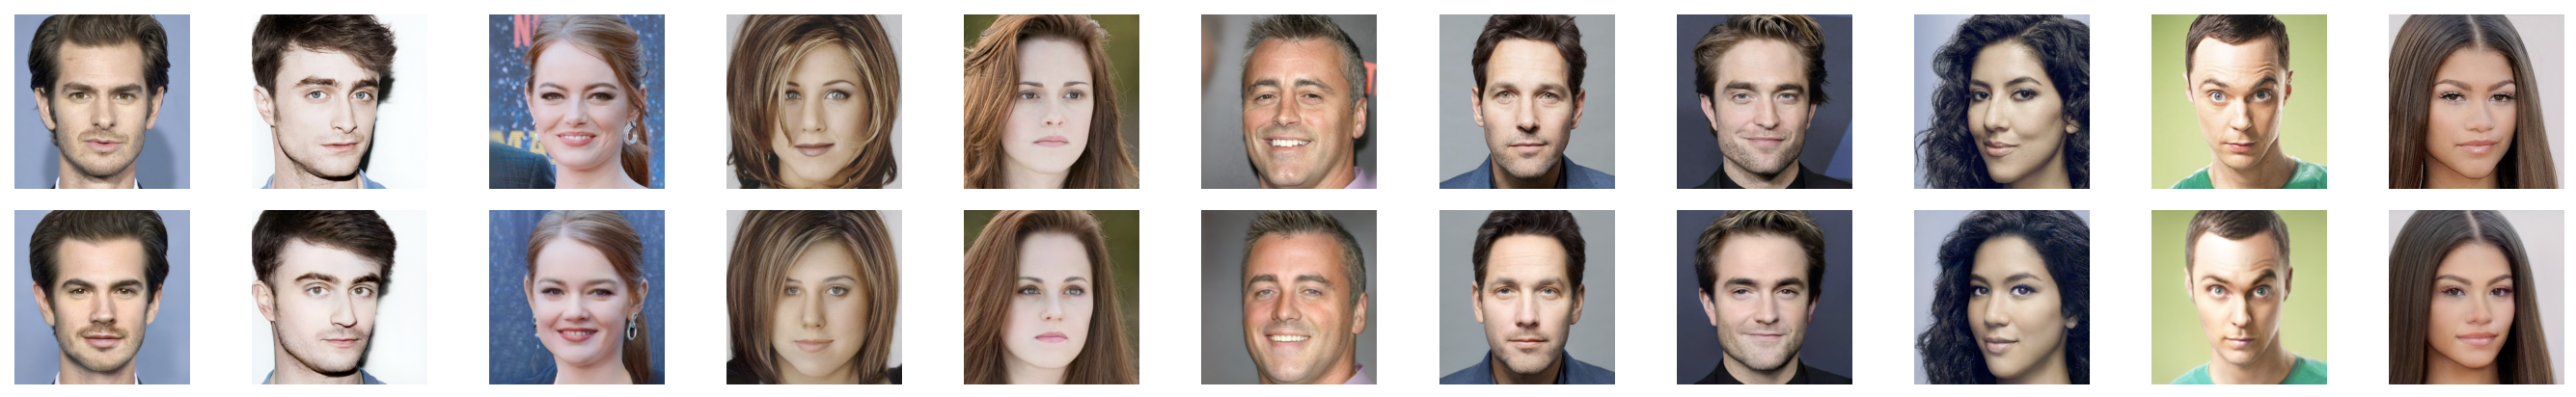
\includegraphics[width=\linewidth, center]{Images/faces_with_projection.png}
  \caption{The 11 chosen faces and their respective projection generated by StyleGAN2 to their bottom.}
  \label{fig:projections}
\end{figure}

\subsection{Correction for projection}

Figure \ref{fig:variation_iterations} illustrates the improvement in the outer facial features difference through the iterations of the correction. The curves of variation significantly decrease in the first 750 iterations. The last 1250 iterations takes account for the last 10\% of the improvement. It is notable that the improvement in the variation is always superior to the 20\% of the initial value, and in some of the cases, it goes over the 50\%. 

\begin{figure}[H]

\begin{subfigure}{0.49\textwidth}
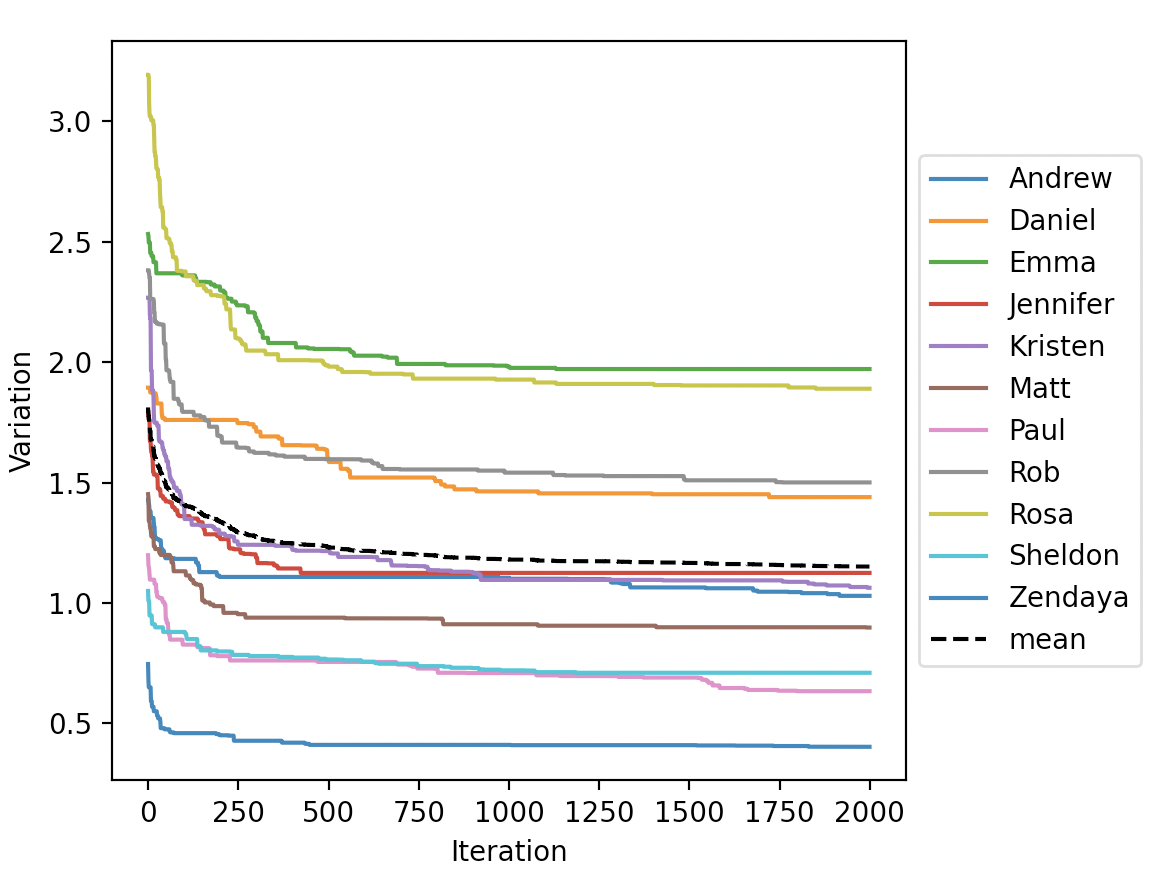
\includegraphics[width=0.9\linewidth]{Images/absolute.png} 
\caption{Absolute}
\label{fig:absolute}
\end{subfigure}
\begin{subfigure}{0.49\textwidth}
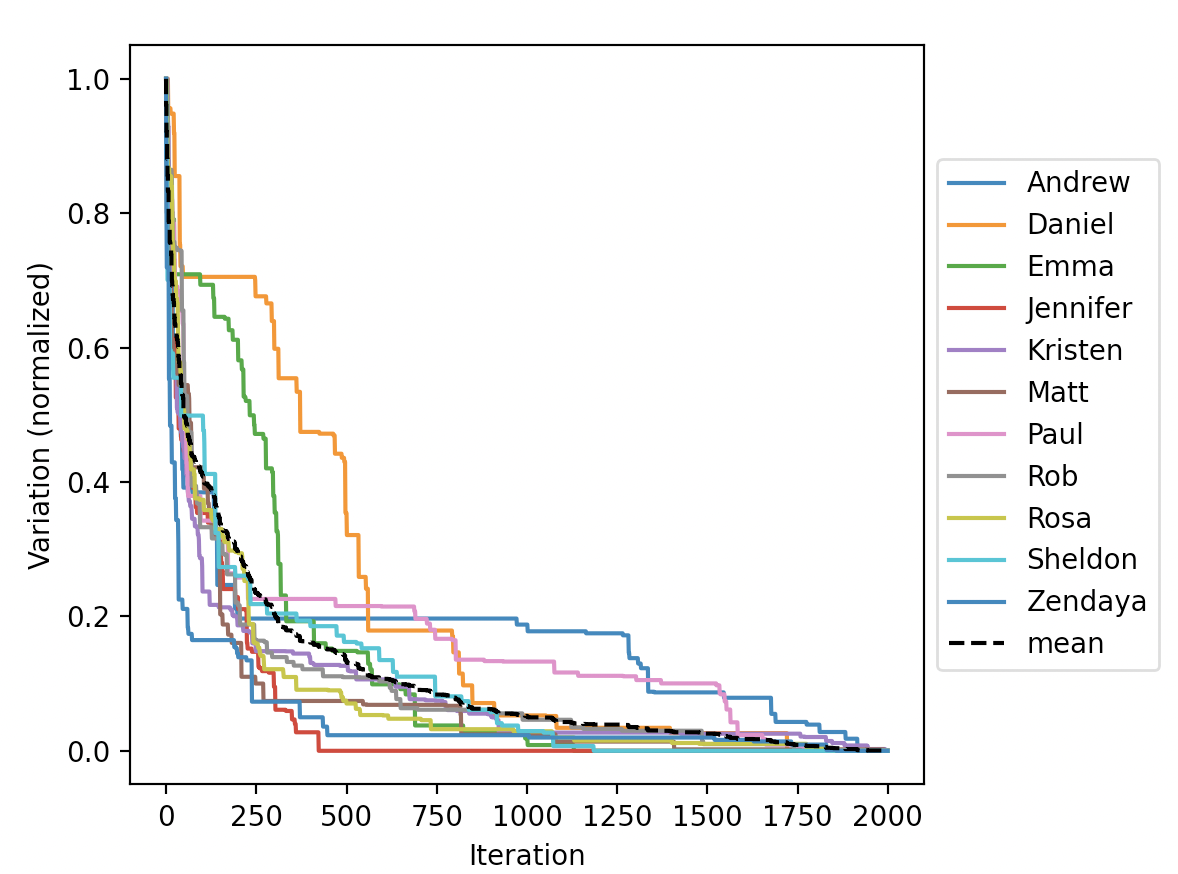
\includegraphics[width=0.9\linewidth]{Images/normalized.png}
\caption{Normalized}
\label{fig:normalized}
\end{subfigure}

\caption{Graphs of the outer facial features difference through iterations}
\label{fig:variation_iterations}
\end{figure}

\subsection{Latent directions}

We also check the outer facial features difference for the 10 images when transforming those moving across the some of the latent directions known by the community~\citep{Luxemburg_2019}. In Figure ~\ref{fig:samples}, we can see the chosen images. They are labeled as 1 to 10 from left to right.

\begin{figure}[H]
  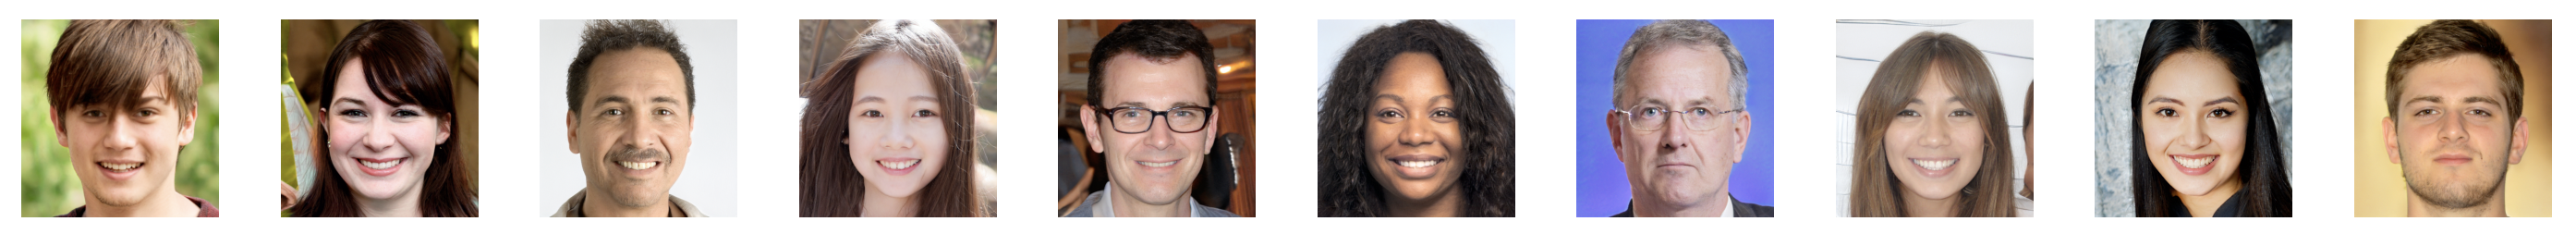
\includegraphics[width=\linewidth, center]{Images/sample_faces.png}
  \caption{The 10 chosen faces for the latent directions experiments.}
  \label{fig:samples}
\end{figure}

When an image moves a great magnitude through a direction, they tend to give unexpected results, deforming the base structure of the face and giving unrealistic images. This is the reason the range measured in each direction changes in each case. For the set of chosen images, we decided the following ranges:

\begin{table}[H]
\centering
\begin{tabular}{|l|l|l|l|l|l|l|l|}
\hline
\textbf{Direction} & Age & Gender & Vertical & Horizontal & Eyes-open & Mouth-open & Smile \\ \hline
\textbf{Range} & [-3, 3] & [-3, 3] & [-3, 3] & [-3, 3] & [-10, 10] & [-10, 10] & [-2, 2] \\ \hline
\end{tabular}
    \caption{Ranges to measure for each direction}
  \label{table:ranges}
\end{table}

Figure \ref{fig:graph_means} shows that the outer facial features difference is directly proportional to the distance moved in every tested direction. Horizontal alignment has the most impact on the outer facial features difference when compared to the others. On the other hand, the mouth and eyes opening directions show the least impact.

% TODO: rehacer grafico normalizando eje x
\begin{figure}[H]
  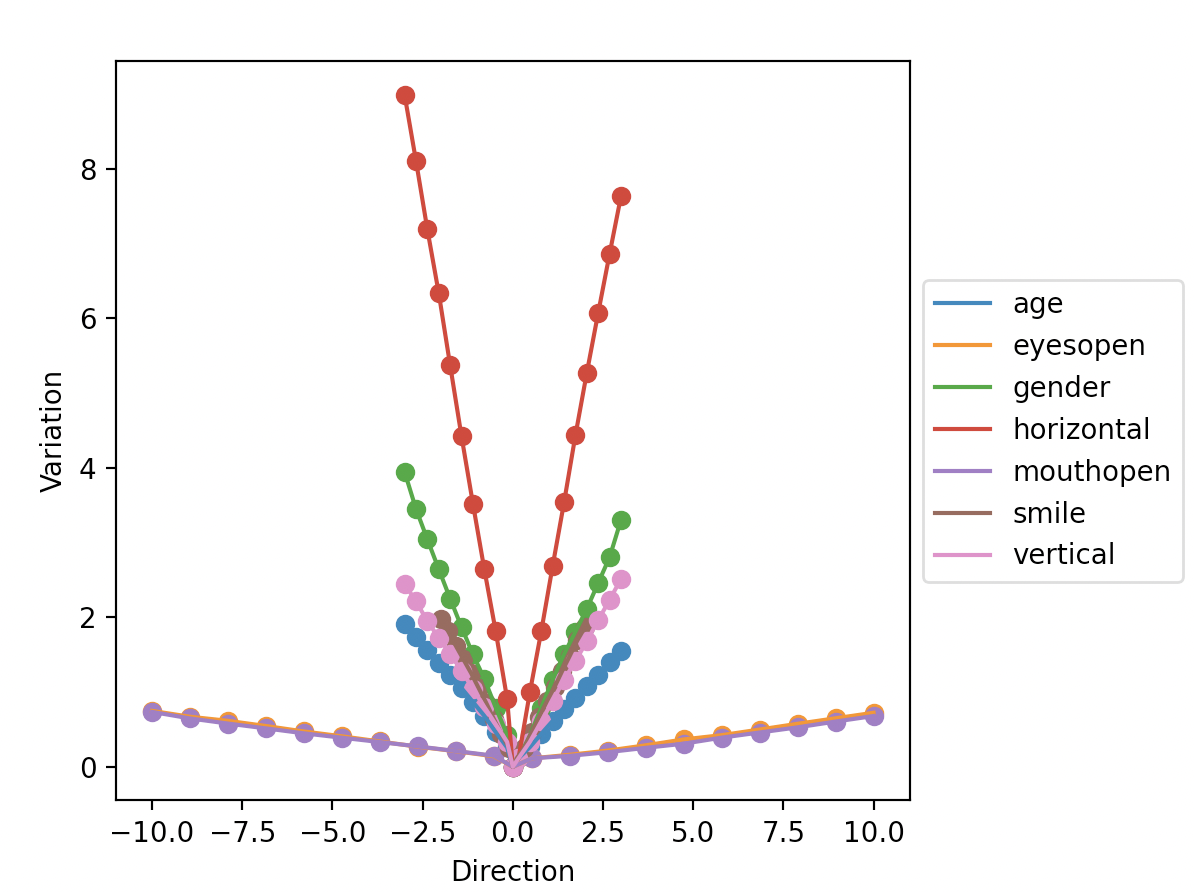
\includegraphics[width=0.8\linewidth, center]{Images/graph_means.png}
  \caption{Graph of the mean outer facial features variations through the each studied direction}
  \label{fig:graph_means}
\end{figure} 

\section{Conclusions}\label{section:conclusions}

After the proposed post-processing step, the measured outer facial features difference always decreased at least 20\% of the initial value. This proves that the proposed algorithm is useful when trying to project a target image generating a new one which is not only similar to the original one in terms of facial characteristics, but it also keeps most of the outer facial features as much as possible.

The outer facial features difference seems to increase with the magnitude of the movement through any of the studied directions in a linear way. However, the rate of such variation is different for each direction. Indicating that there are features that have a bigger influence in the outer facial features than others according to the neural network model.

The proposed work is a step toward better perceived quality in face editing techniques with StyleGAN and the better understanding of the latent space.

FALTAN MUCHAS MAS REFERENCIAS !!!! (Si, siguen faltando :D)


\bibliography{styleganfaceframe}

\end{document}
